\documentclass{article}
\usepackage[T1]{fontenc}
\usepackage[osf]{garamondx}
\usepackage[garamondx,cmbraces]{newtxmath}
\usepackage{fullpage}
\usepackage{wrapfig}
\usepackage{tikz}
\usepackage[backend=biber]{biblatex}

\usetikzlibrary{arrows,shapes,positioning}

\author{Rosemary McCloskey}
\title{M.Sc. Thesis Proposal: Inference of Network Parameters with Kernel-ABC}
\addbibresource{refs.bib}
\begin{document}

\maketitle

\section{Motivation}

\begin{wrapfigure}{R}{0.6\textwidth}
    \centering
    \includegraphics[scale=0.8, trim=0 0 2in 0, clip=true]{transmission.pdf}
    \includegraphics[scale=0.8, trim=0.5in 0 2in 0, clip=true]{transmission_tree.pdf}
    \caption{Correspondence between transmission events (left) and viral
    phylogeny (right).}
    \label{fig:trans}
\end{wrapfigure}

RNA viruses, such as HIV, evolve rapidly within their hosts, accumulating
significant genetic diversity within months of a transmission event. This
process of transmission and subsequent divergent evolution is similar to the
speciation process observed in the evolution of macro-organisms, which often
occurs following the geographic isolation of a sub-population in a new
environment. For both viruses and macro-organisms, these isolation events
roughly correspond to branching points in their ``family tree'', or
\emph{phylogeny}. The relationship between transmissions and viral phylogenies
is illustrated in Figure \ref{fig:trans}, although several complicating factors
prevent the correspondence from being exact.

The practical consequence of this correspondence is the potential to infer
information about transmission patterns from the viral phylogeny. At least
theoretically, phylogenies are easy to construct, and are less susceptible to
biases associated with more conventional methods of investigating transmission
(such as contact tracing). This is the basis for the emerging area of research
known as \emph{phylodynamics}.

Recently, many phylodynamic investigations have been performed aiming to
uncover population-level parameters, such as basic reproductive
number~\cite{stadler2014insights}. Most often, these studies assume a
homogeneously mixed population where contact probabilities between all pairs of
individuals are the same, regardless of geographic or social structure.
However, it is also known that different contact network structures can have
strong effects on epidemic dynamics~\cite{volz2009epidemic}. A small number of
studies have investigated the potential for phylodynamic inference of contact
network structure~\cite{colijn2014phylogenetic,leventhal2012inferring} by
showing that extremely different networks result in differently shaped
phylogenies. I plan to carry this idea further, by identifying parameters of
contact networks which can be effectively estimated with phylodynamic methods
for real, ongoing epidemics.

\section{Methods}

\begin{wrapfigure}{R}{0.6\textwidth}
    \centering
    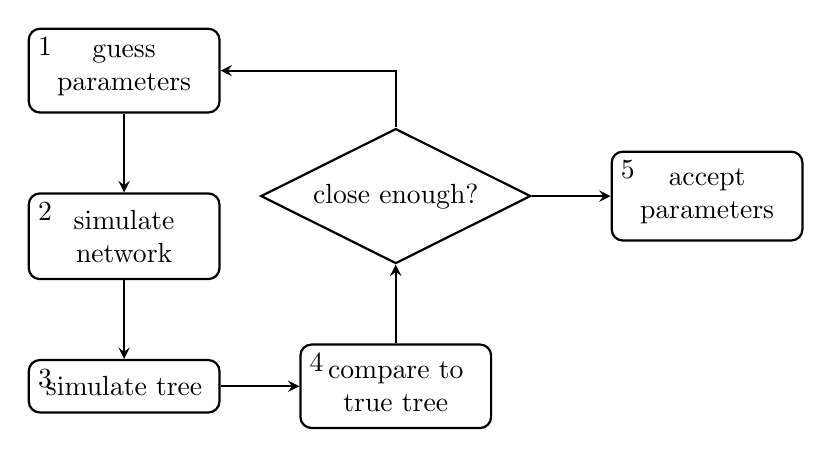
\begin{tikzpicture}
        [state/.style={rounded corners, rectangle, draw, inner sep=6pt, text width=2cm, align=center},
        decision/.style={diamond, aspect=2, draw},
        every path/.style={->, >=stealth, thick}]
        \node[state] (1) {guess parameters};
        \node[state, below=of 1] (2) {simulate network};
        \node[state, below=of 2] (3) {simulate tree};
        \node[state, right=of 3] (4) {compare to true tree};
        \node[decision, above=of 4] (5) {close enough?};
        \node[state, right=of 5] (6) {accept parameters};
        \node at (1.north west) [anchor=north west] {1};
        \node at (2.north west) [anchor=north west] {2};
        \node at (3.north west) [anchor=north west] {3};
        \node at (4.north west) [anchor=north west] {4};
        \node at (6.north west) [anchor=north west] {5};
        \draw (1) -- (2);
        \draw (2) -- (3);
        \draw (3) -- (4);
        \draw (4) -- (5);
        \draw (5.north) |- (1);
        \draw (5) -- (6);
    \end{tikzpicture}
    \caption{Schematic of phylodynamic ABC-rejection algorithm.}
    \label{fig:abc}
\end{wrapfigure}

I propose to use \emph{approximate Bayesian computation} (ABC) to investigate
the contact network structure underlying observed viral phylogenies. ABC
provides a method to estimate the parameters of models without explicit
likelihood calculations, when these are unavailable or computationally
prohibitive. 

To illustrate, I describe the simplest ABC algorithm, called ABC-rejection, as
applied to this problem. A graphical schematic of the algorithm is shown in
Figure~\ref{fig:abc}. The objective of the algorithm is to fit a generative
model for contact networks with a small number of parameters. For example, the
Barabasi-Albert model~\cite{albert2002statistical}, in its simplest form, has
two parameters: the number of nodes in the network ($N$), and the mean degree
of each node in the network ($k$, corresponding to the mean number of contacts
per person). We assume, as is commonly done in phylodynamic studies, that the
true transmission tree is known with certainty.

We begin by guessing a set of parameters (Figure \ref{fig:abc}, box 1), for
example, an at-risk population size of $N = 5000$ with an average of $k = 8$
contacts per person.  A network is generated which satisfies these parameters
(box 2). We then simulate an epidemic over the network, and by keeping track of
who infects who, we derive a simulated transmission tree (box 3). This
simulated tree is compared to the true tree using a phylogenetic
kernel~\cite{poon2013mapping} (box 4). If the simulate tree is sufficiently
similar to the real tree, we accept the model parameters as possibly having
generated the true data (box 5). Otherwise, another set of parameters is
guessed, and we start at the beginning.

In practice, I intend to use either ABC-MCMC or ABC-SMC, rather than this
rejection method. These algorithms have the same basic premise as described
above, but use more sophisticated methods of ``guessing'' parameters, to reduce
the number of iterations needed to converge to the true values.

\section{Progress}

I have implemented a method to simulate transmission trees over networks, and
partially validated it by reconstructing Figure 1a
from~\cite{leventhal2012inferring}, which examined the effect of network type
(scale-free vs. small-world vs. random) on a particular tree summary statistic
(Sackin's index). As a proof of concept, I used the same parameters as in that
paper to develop a tree kernel-based classifier for tree shape, which was
94.6\% accurate at classifying the network type underlying simulated
phylogenies (Figure \ref{fig:kmat}).

\section{Goals}

The schematic in Figure \ref{fig:abc} outlines five major tasks required for
this project.

\begin{enumerate}
    \item Decide how to parameterize contact networks, and what sorts of
        parameters are both useful and feasible to infer.
    \item Simulate contact networks from a generative model. Several
        out-of-the-box graph generators exist (eg. for scale-free, small-world,
        and random graphs), but may need to be adapted depending on the
        generative model.
    \item Simulate phylogenies over contact networks. This has already been
        done.
    \item Compare simulated to observed phylogenies. I will use the tree
        kernel~\cite{poon2013mapping} for this task, which has an existing
        implementation.
    \item Implement the overall algorithm for proposing and accepting
        parameters, in other words, ABC-SMC or ABC-MCMC.
\end{enumerate}

\begin{figure}
    \centering
    \includegraphics[trim=0 0 0 0, clip=true, scale=0.5]{kmat.pdf}
    \label{fig:kmat}
    \caption{Principal components projection of kernel matrix of 300 simulated
    trees from three different network types.}
\end{figure}
\printbibliography

\end{document}
